\newpage
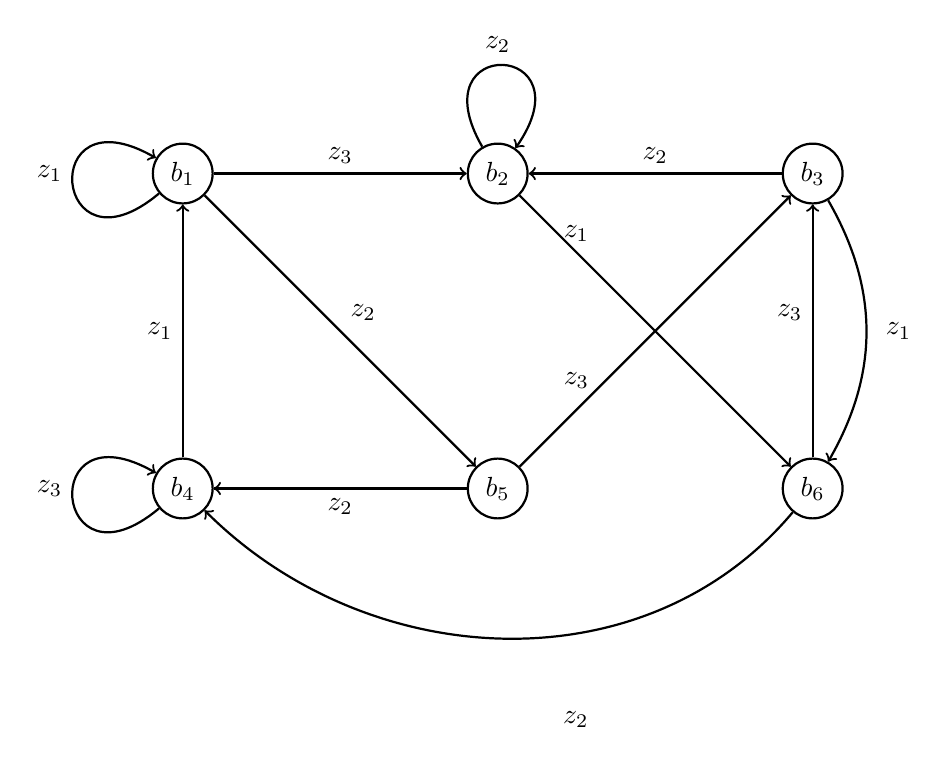
\begin{tikzpicture}[node distance={40mm}, thick, main/.style = {draw, circle}] 
\node[main] (1) {$b_1$}; 
\node[main] (2) [right of=1] {$b_2$};
\node[main] (3) [right of=2] {$b_3$};
\node[main] (4) [below of=1] {$b_4$};
\node[main] (5) [below of=2] {$b_5$};
\node[main] (6) [below of=3] {$b_6$};
\draw[->] (1) to [out=220,in=150,looseness=10] (1); 
\draw[->] (1) -- node[midway,above] {$z_3$} (2);
\draw[->] (2) to [out=120,in=55,looseness=10] (2);
\draw[->] (4) to [out=220,in=150,looseness=10] (4);
\draw[->] (6) to [out=230, in=315, looseness=1] (4);
\draw[->] (3) to [out=300, in=60, looseness=1] (6);
\draw[->] (3) -- node[midway,above] {$z_2$} (2);
\draw[->] (2) -- node[above left=1cm, above] {$z_1$} (6);
\draw[->] (4) -- node[midway,left] {$z_1$} (1);
\draw[->] (1) -- node[midway, above right] {$z_2$} (5);
\draw[->] (5) -- node[left=1cm,below=0.4cm] {$z_3$} (3);
\draw[->] (5) -- node[midway,below] {$z_2$} (4); 
\draw[->] (6) -- node[midway, above left] {$z_3$} (3);
\draw (2) -- node[above=1.4cm] {$z_2$} (2);
\draw (1) -- node[left=1.4cm] {$z_1$} (1);
\draw (4) -- node[left=1.4cm] {$z_3$} (4);
\draw (5) -- node[below right=2.7cm] {$z_2$} (4);
\draw (6) -- node[right=0.8cm] {$z_1$} (3);
\end{tikzpicture}